% Options for packages loaded elsewhere
\PassOptionsToPackage{unicode}{hyperref}
\PassOptionsToPackage{hyphens}{url}
%
\documentclass[
]{article}
\title{final-project}
\author{Pragyat Agrawal \and Ruxuan Ji \and Meng-Chuan Chang}
\date{}

\usepackage{amsmath,amssymb}
\usepackage{lmodern}
\usepackage{iftex}
\ifPDFTeX
  \usepackage[T1]{fontenc}
  \usepackage[utf8]{inputenc}
  \usepackage{textcomp} % provide euro and other symbols
\else % if luatex or xetex
  \usepackage{unicode-math}
  \defaultfontfeatures{Scale=MatchLowercase}
  \defaultfontfeatures[\rmfamily]{Ligatures=TeX,Scale=1}
\fi
% Use upquote if available, for straight quotes in verbatim environments
\IfFileExists{upquote.sty}{\usepackage{upquote}}{}
\IfFileExists{microtype.sty}{% use microtype if available
  \usepackage[]{microtype}
  \UseMicrotypeSet[protrusion]{basicmath} % disable protrusion for tt fonts
}{}
\makeatletter
\@ifundefined{KOMAClassName}{% if non-KOMA class
  \IfFileExists{parskip.sty}{%
    \usepackage{parskip}
  }{% else
    \setlength{\parindent}{0pt}
    \setlength{\parskip}{6pt plus 2pt minus 1pt}}
}{% if KOMA class
  \KOMAoptions{parskip=half}}
\makeatother
\usepackage{xcolor}
\IfFileExists{xurl.sty}{\usepackage{xurl}}{} % add URL line breaks if available
\IfFileExists{bookmark.sty}{\usepackage{bookmark}}{\usepackage{hyperref}}
\hypersetup{
  pdftitle={final-project},
  pdfauthor={Pragyat Agrawal; Ruxuan Ji; Meng-Chuan Chang},
  hidelinks,
  pdfcreator={LaTeX via pandoc}}
\urlstyle{same} % disable monospaced font for URLs
\usepackage[margin=1in]{geometry}
\usepackage{color}
\usepackage{fancyvrb}
\newcommand{\VerbBar}{|}
\newcommand{\VERB}{\Verb[commandchars=\\\{\}]}
\DefineVerbatimEnvironment{Highlighting}{Verbatim}{commandchars=\\\{\}}
% Add ',fontsize=\small' for more characters per line
\usepackage{framed}
\definecolor{shadecolor}{RGB}{248,248,248}
\newenvironment{Shaded}{\begin{snugshade}}{\end{snugshade}}
\newcommand{\AlertTok}[1]{\textcolor[rgb]{0.94,0.16,0.16}{#1}}
\newcommand{\AnnotationTok}[1]{\textcolor[rgb]{0.56,0.35,0.01}{\textbf{\textit{#1}}}}
\newcommand{\AttributeTok}[1]{\textcolor[rgb]{0.77,0.63,0.00}{#1}}
\newcommand{\BaseNTok}[1]{\textcolor[rgb]{0.00,0.00,0.81}{#1}}
\newcommand{\BuiltInTok}[1]{#1}
\newcommand{\CharTok}[1]{\textcolor[rgb]{0.31,0.60,0.02}{#1}}
\newcommand{\CommentTok}[1]{\textcolor[rgb]{0.56,0.35,0.01}{\textit{#1}}}
\newcommand{\CommentVarTok}[1]{\textcolor[rgb]{0.56,0.35,0.01}{\textbf{\textit{#1}}}}
\newcommand{\ConstantTok}[1]{\textcolor[rgb]{0.00,0.00,0.00}{#1}}
\newcommand{\ControlFlowTok}[1]{\textcolor[rgb]{0.13,0.29,0.53}{\textbf{#1}}}
\newcommand{\DataTypeTok}[1]{\textcolor[rgb]{0.13,0.29,0.53}{#1}}
\newcommand{\DecValTok}[1]{\textcolor[rgb]{0.00,0.00,0.81}{#1}}
\newcommand{\DocumentationTok}[1]{\textcolor[rgb]{0.56,0.35,0.01}{\textbf{\textit{#1}}}}
\newcommand{\ErrorTok}[1]{\textcolor[rgb]{0.64,0.00,0.00}{\textbf{#1}}}
\newcommand{\ExtensionTok}[1]{#1}
\newcommand{\FloatTok}[1]{\textcolor[rgb]{0.00,0.00,0.81}{#1}}
\newcommand{\FunctionTok}[1]{\textcolor[rgb]{0.00,0.00,0.00}{#1}}
\newcommand{\ImportTok}[1]{#1}
\newcommand{\InformationTok}[1]{\textcolor[rgb]{0.56,0.35,0.01}{\textbf{\textit{#1}}}}
\newcommand{\KeywordTok}[1]{\textcolor[rgb]{0.13,0.29,0.53}{\textbf{#1}}}
\newcommand{\NormalTok}[1]{#1}
\newcommand{\OperatorTok}[1]{\textcolor[rgb]{0.81,0.36,0.00}{\textbf{#1}}}
\newcommand{\OtherTok}[1]{\textcolor[rgb]{0.56,0.35,0.01}{#1}}
\newcommand{\PreprocessorTok}[1]{\textcolor[rgb]{0.56,0.35,0.01}{\textit{#1}}}
\newcommand{\RegionMarkerTok}[1]{#1}
\newcommand{\SpecialCharTok}[1]{\textcolor[rgb]{0.00,0.00,0.00}{#1}}
\newcommand{\SpecialStringTok}[1]{\textcolor[rgb]{0.31,0.60,0.02}{#1}}
\newcommand{\StringTok}[1]{\textcolor[rgb]{0.31,0.60,0.02}{#1}}
\newcommand{\VariableTok}[1]{\textcolor[rgb]{0.00,0.00,0.00}{#1}}
\newcommand{\VerbatimStringTok}[1]{\textcolor[rgb]{0.31,0.60,0.02}{#1}}
\newcommand{\WarningTok}[1]{\textcolor[rgb]{0.56,0.35,0.01}{\textbf{\textit{#1}}}}
\usepackage{graphicx}
\makeatletter
\def\maxwidth{\ifdim\Gin@nat@width>\linewidth\linewidth\else\Gin@nat@width\fi}
\def\maxheight{\ifdim\Gin@nat@height>\textheight\textheight\else\Gin@nat@height\fi}
\makeatother
% Scale images if necessary, so that they will not overflow the page
% margins by default, and it is still possible to overwrite the defaults
% using explicit options in \includegraphics[width, height, ...]{}
\setkeys{Gin}{width=\maxwidth,height=\maxheight,keepaspectratio}
% Set default figure placement to htbp
\makeatletter
\def\fps@figure{htbp}
\makeatother
\setlength{\emergencystretch}{3em} % prevent overfull lines
\providecommand{\tightlist}{%
  \setlength{\itemsep}{0pt}\setlength{\parskip}{0pt}}
\setcounter{secnumdepth}{5}
\ifLuaTeX
  \usepackage{selnolig}  % disable illegal ligatures
\fi

\begin{document}
\maketitle

{
\setcounter{tocdepth}{3}
\tableofcontents
}
\hypertarget{executive-summary}{%
\section{Executive Summary}\label{executive-summary}}

\hypertarget{background}{%
\subsection{Background}\label{background}}

The US rental market has been growing rapidly growing over time, making
it one of the most sought after areas for investment. Be it from small
home owners to big private equity firms, everyone seems to be after
housing, expecting the values of these houses to rise and supplement
their income by renting these places. Many people consider that location
is the ``only important'' factor responsible for a house's value and the
rent that can be expected of it, but this is far from the truth. There
are a lot of other factors that need to be considered for determining
housing valuations as we see a huge variation in prices in houses
located in the same vicinity. There must be something about these houses
which is causing such a big price change. Hence we will be analyzing the
data related to US Rental Listings in Summer of 2021, to find which of
these factors, which consist of many in-house amenity components,
impacts housing values the most.

These amenities range from simple aka micro-factors like the
availability of Pools and Dishwashers in the house to major aka
macro-factors i.e.~cities. The data will also give us the opportunity to
find in which cities are these factors playing the most impact. With
over 27,000 values for each predictor in our data, we have a sufficient
sample size to make a reasonable conclusion regarding the price of these
summer rentals.

Graph: Rental vacancy rates in the United States from 2000 to 2021, by
region (Source: Statista.com)

This shows how the US housing market has been more sought after year by
year, making housing a form of valuable investment. This increase in
demand has already pushed up the prices.

\begin{figure}

{\centering 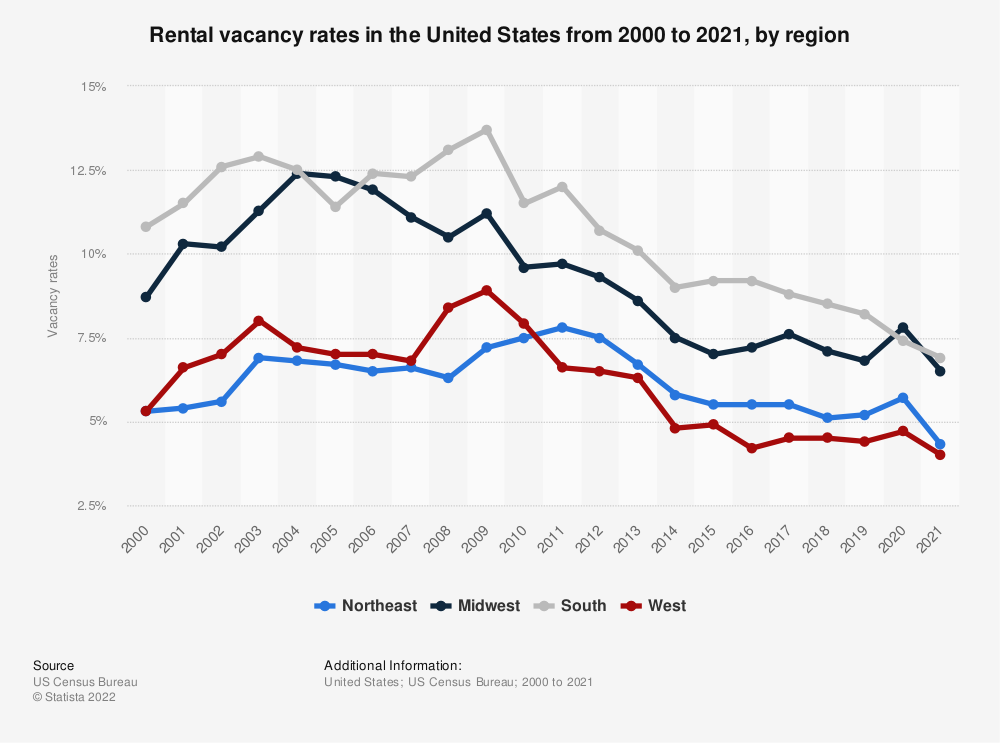
\includegraphics[width=1\linewidth]{image/rental-vacancy-rates} 

}

\caption{A caption}\label{fig:pressure}
\end{figure}

\hypertarget{description-of-data}{%
\subsection{Description of Data}\label{description-of-data}}

The data is gathered from Kaggle, a huge repository of community
published code and data. This data was pulled from Rentler.com on
7/12/2021, 8/12/2021, and 9/6/2021, and population density data was
scraped by zip code from mapszipcode.com on 7/12/2021. The pull from
Rentler.com resulted in 4 CSV files which included the main rental
listing, the list of amenities, the list of lease terms, and a list of
who was responsible to pay each utility. Many of the variables that were
sparsely populated were dropped before denormalizing the dataset. The
rental listing information was joined with the population and population
density information from mapszipcode.com (Source: Kaggle). Many of the
data columns in the dataset are embedded in binary format with 0
representing the absence of the predictor attribute while 1, shows that
the attribute is present. The data file is massive at around half a
Gigabyte. Working with this size of data, we would have to use EDA or
take a subset of the dataset for R to run effectively and not crash over
the large size of the data. We will explore this idea in later sections.
For now, the data is sufficient for analysis.

Our response variable is PRICE which represents the monthly price for
the particular summer listing on rental.com.

\begin{table}[!h]
\centering
\caption{Variables and their descriptions}
\begin{tabular}{cc}
\hline 
Variable & Description\tabularnewline
\hline 
V1 & Numbering for the house number we are looking at (form of house identification)\tabularnewline
pool & Binary data to show if pool exists in this house (1) or not (0)\tabularnewline
dishwasher & Binary data to show if dishwasher exists in the house (1) or not (0)\tabularnewline
washer-dryer & Binary data to show if washer-dryer exists in the house(1) or not (0)\tabularnewline
ac & Binary data to show if air conditioning exists in the house (1) or not (0)\tabularnewline
parking & Binary data to show if Parking exists in the house (1) or not (0)\tabularnewline
zip & Zip code of the property\tabularnewline
price & Monthly rent price for the property\tabularnewline
city & City where the property is located\tabularnewline
num\_beds & Number of beds in the property\tabularnewline
num\_baths & Number of baths in the property\tabularnewline
house\_type & Type of house we are looking at\tabularnewline
sqft & Square Feet in the property\tabularnewline
smoking\_ind & Does the rental allow smoking (Yes/No) \tabularnewline
pets\_ind & Does the rental allow pets (Yes/No)\tabularnewline
acres & Number of acres rental includes\tabularnewline
description & 4000 character listing description of the rental\tabularnewline
ZipCity & Primary city for the zip code\tabularnewline
Population & Population in the zip code\tabularnewline
PopulationDensity & Population density per square mile for zip code\tabularnewline
security\_deposit & Security deposit required\tabularnewline
\hline 
\end{tabular}
\label{lyxtab2}
\end{table}

\hypertarget{goal}{%
\subsection{Goal}\label{goal}}

The goal of this study is to analyze the most important factors
affecting the housing prices in the US. We will be using the variables
in the dataset to do so. In our preliminary market analysis, we found
that housing prices are determined by many factors and hence we will try
to ascertain factors which have a significant impact on housing prices.
Our goal is to build a model that will give us the value added or
subtracted from a house with/without the presence of a variable factor.
This observation will benefit people who are looking to rent properties
in the US and can help them get a better value for the kind of place
they may be looking for.

\hypertarget{summary-of-findings}{%
\subsection{Summary of Findings}\label{summary-of-findings}}

\hypertarget{issues-and-limitations}{%
\subsection{Issues and Limitations}\label{issues-and-limitations}}

The biggest issue we initially faced was with respect to the file size
which turned out to be quiet massive even for R Studio. The raw data we
started with was half a gigabyte big which turned out to be very massive
for any for of extrapolation. Hence we had to shorten the data
out\ldots\ldots.

\hypertarget{exploratory-data-analysis}{%
\section{Exploratory Data Analysis}\label{exploratory-data-analysis}}

\hypertarget{data-preprocessingcleaning}{%
\subsection{Data
Preprocessing/Cleaning}\label{data-preprocessingcleaning}}

\hypertarget{read-the-data}{%
\subsubsection{Read the data}\label{read-the-data}}

Firstly, we read the data from Kaggle -
\href{https://www.kaggle.com/datasets/elizabethveillon/us-rental-listings-summer-2021}{US
Rental Listings Summer 2021}

\begin{Shaded}
\begin{Highlighting}[]
\NormalTok{data }\OtherTok{\textless{}{-}} \FunctionTok{fread}\NormalTok{(}\StringTok{"data/Rental\_Properties.csv"}\NormalTok{)}
\FunctionTok{summary}\NormalTok{(data)}
\end{Highlighting}
\end{Shaded}

\hypertarget{filter-the-data}{%
\subsubsection{Filter the data}\label{filter-the-data}}

The original dataset contains 276757 data, but we just need partial
data. Before we randomly pick 20000 for further analysis, we can remove
rows that is lack of important factors. The criteria is as follows

\begin{itemize}
\tightlist
\item
  sqft (squart feet) must be non-zero
\item
  population and the density must be non-zero
\item
  price must be non-zero
\end{itemize}

\begin{Shaded}
\begin{Highlighting}[]
\NormalTok{data\_filter }\OtherTok{\textless{}{-}}\NormalTok{ data[(data}\SpecialCharTok{$}\NormalTok{sqft}\SpecialCharTok{!=}\DecValTok{0} \SpecialCharTok{\&}\NormalTok{ data}\SpecialCharTok{$}\NormalTok{Population}\SpecialCharTok{!=}\DecValTok{0}\NormalTok{),]}
\NormalTok{data\_filter }\OtherTok{\textless{}{-}}
\NormalTok{  data\_filter }\SpecialCharTok{\%\textgreater{}\%}
  \FunctionTok{drop\_na}\NormalTok{(price)}
\FunctionTok{set.seed}\NormalTok{(}\DecValTok{1}\NormalTok{)}
\NormalTok{data\_20000 }\OtherTok{\textless{}{-}} \FunctionTok{sample\_n}\NormalTok{(data\_filter, }\DecValTok{20000}\NormalTok{)}
\end{Highlighting}
\end{Shaded}

Then we drop several columns which is clearly not helpful for predicting
the rental price

\begin{itemize}
\tightlist
\item
  link
\item
  street\_address
\item
  full\_address
\end{itemize}

\begin{Shaded}
\begin{Highlighting}[]
\NormalTok{data\_20000\_filter }\OtherTok{\textless{}{-}}
\NormalTok{  data\_20000 }\SpecialCharTok{\%\textgreater{}\%}
  \FunctionTok{select}\NormalTok{(}\SpecialCharTok{{-}}\NormalTok{link, }\SpecialCharTok{{-}}\NormalTok{street\_address, }\SpecialCharTok{{-}}\NormalTok{full\_address)}
\end{Highlighting}
\end{Shaded}

Finally, we fill all NA with 0. The columns having NA is as follows

\begin{itemize}
\tightlist
\item
  pool
\item
  dishwasher
\item
  washer-dryer
\item
  ac
\item
  parking
\item
  zip
\item
  ZipCity
\end{itemize}

Then we export the cleaned dataframe to csv

\begin{Shaded}
\begin{Highlighting}[]
\NormalTok{data\_20000\_filter[}\FunctionTok{is.na}\NormalTok{(data\_20000\_filter)] }\OtherTok{\textless{}{-}} \DecValTok{0}
\FunctionTok{summary}\NormalTok{(data\_20000\_filter)}

\NormalTok{file\_path }\OtherTok{\textless{}{-}} \StringTok{"data/Rental\_Properties\_20000.csv"}

\ControlFlowTok{if}\NormalTok{(}\SpecialCharTok{!}\FunctionTok{file.exists}\NormalTok{(file\_path)) \{}
  \FunctionTok{write.csv}\NormalTok{(data\_20000\_filter, file\_path)}
\NormalTok{\} }\ControlFlowTok{else}\NormalTok{ \{}
\NormalTok{  data\_20000\_filter }\OtherTok{\textless{}{-}} \FunctionTok{fread}\NormalTok{(file\_path)}
\NormalTok{\}}
\end{Highlighting}
\end{Shaded}

\hypertarget{data-transformations-and-plots}{%
\subsection{Data Transformations and
Plots}\label{data-transformations-and-plots}}

\begin{center}\includegraphics{final-project_files/figure-latex/unnamed-chunk-1-1} \end{center}

house\_type n 1: Apartment 17749 2: Condo/Multiplex 1519 3: House 219 4:
In-Law/Basement 26 5: Single Room 211 6: Sublease or Student Contract 1
7: Townhome 275

Looking at the data we see that the properties we will most be
evaluating will be Apartment style places with 17749 observations. Other
places are lesser in number but still there. The second largest group is
the Condo/Multiplex group that we are looking at with 1519 observations.
Other than that the smallest group we see is the sublease or student
contract group which only has 1 observation.

\begin{center}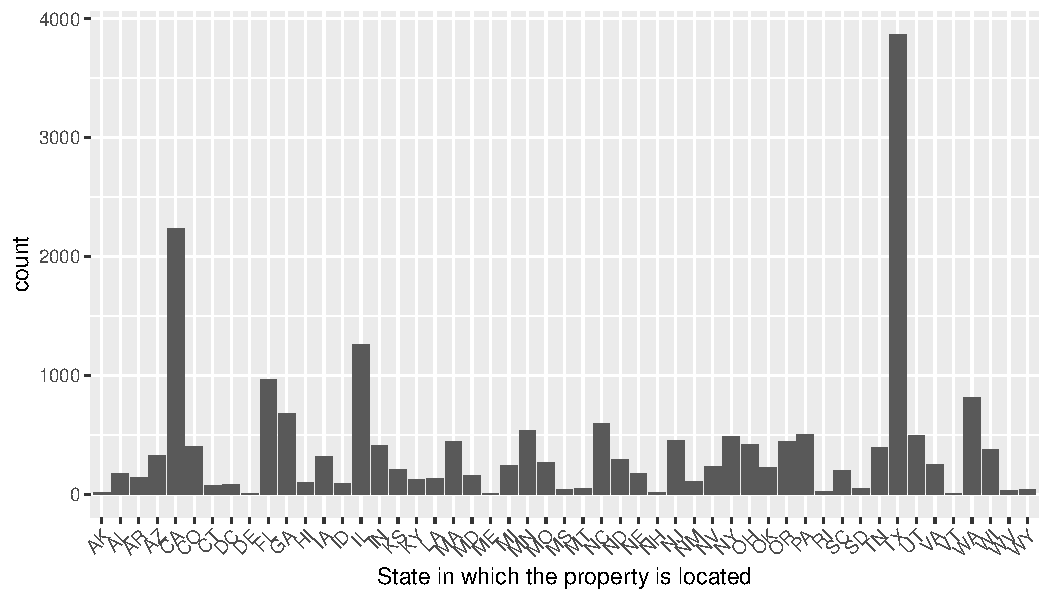
\includegraphics{final-project_files/figure-latex/unnamed-chunk-3-1} \end{center}

\begin{Shaded}
\begin{Highlighting}[]
\NormalTok{number\_states }\OtherTok{\textless{}{-}}\NormalTok{ data\_20000\_filter }\SpecialCharTok{\%\textgreater{}\%}
  \FunctionTok{group\_by}\NormalTok{(state) }\SpecialCharTok{\%\textgreater{}\%} \FunctionTok{count}\NormalTok{() }

\FunctionTok{arrange}\NormalTok{(number\_states, }\SpecialCharTok{{-}}\NormalTok{n)}
\end{Highlighting}
\end{Shaded}

\begin{verbatim}
## # A tibble: 51 x 2
## # Groups:   state [51]
##    state     n
##    <chr> <int>
##  1 TX     3869
##  2 CA     2238
##  3 IL     1261
##  4 FL      969
##  5 WA      817
##  6 GA      680
##  7 NC      596
##  8 MN      535
##  9 PA      500
## 10 UT      499
## # ... with 41 more rows
\end{verbatim}

The data represents all states, some more than others. Texas is the most
represented state with the least being Vermont at 4 listings. The sample
is representative of all states in the US. We are randomly choosing
20,000 data points so this will fluctuate if we change the data seed.

\begin{Shaded}
\begin{Highlighting}[]
\NormalTok{data\_20000\_filter }\SpecialCharTok{\%\textgreater{}\%} 
  \FunctionTok{ggplot}\NormalTok{(}\FunctionTok{aes}\NormalTok{(}\AttributeTok{x =} \FunctionTok{reorder}\NormalTok{(state,price), }\AttributeTok{y =}\NormalTok{ price ,}\AttributeTok{group=}\NormalTok{state))}\SpecialCharTok{+}
  \FunctionTok{ylim}\NormalTok{ (}\DecValTok{0}\NormalTok{, }\DecValTok{10000}\NormalTok{) }\SpecialCharTok{+} 
  \FunctionTok{xlab}\NormalTok{(}\StringTok{\textquotesingle{}State\textquotesingle{}}\NormalTok{)}\SpecialCharTok{+}
  \FunctionTok{geom\_boxplot}\NormalTok{()}\SpecialCharTok{+}
  \FunctionTok{theme}\NormalTok{(}\AttributeTok{axis.text.x =} \FunctionTok{element\_text}\NormalTok{(}\AttributeTok{angle =} \DecValTok{45}\NormalTok{, }\AttributeTok{vjust =} \DecValTok{1}\NormalTok{, }\AttributeTok{hjust =} \DecValTok{1}\NormalTok{)) }\SpecialCharTok{+}
  \FunctionTok{ggtitle}\NormalTok{(}\StringTok{"Within State Variability of Log Death Rate"}\NormalTok{)}\SpecialCharTok{+}
  \FunctionTok{ylab}\NormalTok{(}\StringTok{"Monthly rent (in $)"}\NormalTok{)}
\end{Highlighting}
\end{Shaded}

\begin{center}\includegraphics{final-project_files/figure-latex/unnamed-chunk-5-1} \end{center}

We see the prices remaining fairly same for the start with the prices
rising with states like New York, California, Florida and Massachusetts.
This is evidently true for these ``more expensive'' places as states on
the right end of the spectrum like California, and Massachusetts are
known for their high per capita incomes which tends to push housing
prices up. There is a lot of variation in data as well as we move to
states with higher housing prices, indicated through the presence of
excessive outliers on the right end of the boxplot.

\hypertarget{model-training}{%
\section{Model Training}\label{model-training}}

\hypertarget{performance-analysis}{%
\section{Performance Analysis}\label{performance-analysis}}

\hypertarget{conclusion}{%
\section{Conclusion}\label{conclusion}}

\end{document}
